\chapter{Theory}
\label{chap:Theory}
%
\section{From Statistical Mechanics to Vacancy configuration} In later chapters only discrete configurations of the system at hand will be examined. Going form a continuos picture of classical phase space to a descrete description is straight forward.First we consider the system of the crystal of Neon Atoms as a canonical ensemble, this means it will be described under the assumption of an infinitely large heat bath by Boltzmann statistics. The probability distribution of members of the ensemble will then be 
\begin{align}
	p(\vec{\mathbf{q}},\vec{\mathbf{p}})=\frac{e^{-\beta H(\vec{\mathbf{q}},\vec{\mathbf{p}})}}{\int\cdots\int e^{-\beta H(\vec{\mathbf{q}},\vec{\mathbf{p}})}\mathrm{d}^{3N}\vec{\mathbf{q}}\mathrm{d}^{3N}\vec{\mathbf{p}}},
\end{align}
with $N$ being the number total of particles of the system.\\\\
Now an ensemble is to be understood as many fictional copies of the same system representing the states that a system will explore when propagating in time according to Hamilton's equation of motion. The ensemble distribution represents the relative number of times that an ergodic system will come by a given state after an infinite amount of time has passed. Now for a crystal in principle this still holds. At low temperatures though the phase space that is being explored can be abstracted in such cases. The reason is that the system will for a given finite time usually explore only nearby points in the phase space. This is the crystal configuration but allowing for dynamics such as lattice vibrations and thermal movement of the atoms with respect to their lattice site. So for a given initial point in phase space the system will mostly explore its proximity until it probabilistically jumps to another volume of phase space whose proximity then will be explored for some further time. Now this means the systems lattice configuration has changed which at low but non zero temperature should be reasonable. 
We now consider these volumes of phase space (being approximately confined regions, i.e. configurations of e.g. a crystalline structure) to be discrete states that the system can be in. So our canonical distribution now is a discrete one, each state representing such a configuration volume. What's left is to figure out what state of the still continuously possible states inside will be used to represent each configuration. We in this work will use the state $(\vec{\mathbf{q}}_{0i},\vec{\mathbf{p}}_{0i})$ that locally minimizes $H(\vec{\mathbf{q}},\vec{\mathbf{p}})$. The Boltzmann distribution now follows to be discrete:
\begin{align}
	p(\vec{\mathbf{q}}_{0i},\vec{\mathbf{p}}_{0i})=\frac{e^{-\beta H(\vec{\mathbf{q}}_{0i},\vec{\mathbf{p}}_{0i})}}{\sum_{n} e^{-\beta H(\vec{\mathbf{q}}_{0n},\vec{\mathbf{p}}_{0n})}}.
\end{align}
Since we know that the momenta $\vec{\mathbf{p}}$ only show up in the kinetic term of the Hamiltonian, we can immediately say that the momenta $\vec{\mathbf{p}}_{0i}$ representing the minimal hamiltonian will be 0 for all possible configurations $(\vec{\mathbf{q}}_{0i},\vec{\mathbf{p}}_{0i})$, so we could just drop the $\vec{\mathbf{p}}$ dependency from here on, but for now we'll continue to write them for completeness and only later on will remember this argument.

\begin{figure}
	\centering
	%trim = left bottom right top
	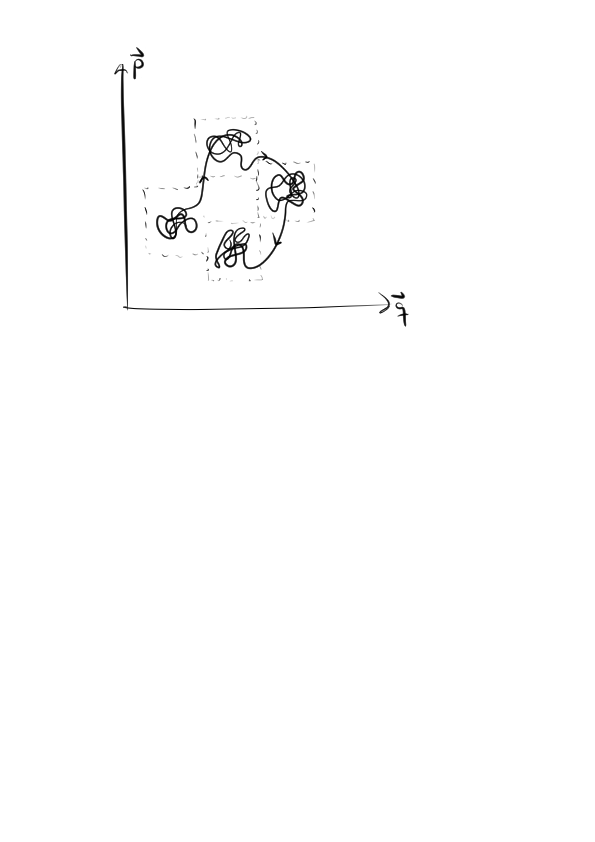
\includegraphics[trim=3cm 18cm 6cm 1.5cm, clip,scale=0.7]{./Inhalt/Bilder/phasespace.png}
	\caption{state evolution $(\vec{\mathbf{q}}(t),\vec{\mathbf{p}}(t))$ through 6N-dimensional phase space}
	\label{fig:phasepsace}
\end{figure}
Now for the problem at hand we will switch to the grand canonical sum, since wee need to introduce two more degrees of freedom, i.e. the particle exchange with the heat and particle bath, which here in general involves two types of particles numbers $N_1,N_2$. They naturally introduce only discrete degrees of freedom so we can quickly write the grand canonical distribution for the system:
\begin{align}
	\rho(N_1,N_2,\vec{\mathbf{q}}_{0i},\vec{\mathbf{p}}_{0i})&=\frac{e^{-\beta\left(H_{N_1N_2}(\vec{\mathbf{q}}_{0i},\vec{\mathbf{p}}_{0i})-\sum_{i=1}^{2}\mu_i N_i\right)}}{\frac{1}{h^{3N}\prod_{j=1}^{2}N_j!}\sum_{N_1}\sum_{N_2}\sum_{n}\left[H_{N_1N_2}(\vec{\mathbf{q}}_{0n},\vec{\mathbf{p}}_{0n})-\sum_{i=1}^{2}\mu_i N_i\right]}=\\
	&=\frac{e^{-\beta\left(H_{N_1N_2}(\vec{\mathbf{q}}_{0i},\vec{\mathbf{p}}_{0i})-\sum_{i=1}^{2}\mu_i N_i\right)}}{\Xi_{\mu_1\mu_2}(T,V)},
\end{align}
with 
\begin{align}
\mu_i = -T \frac{\partial S}{\partial N_i}=\frac{\partial E}{\partial N_i}.
\end{align} the $i$-th chemical potential.
The most probable states $(N_1,N_2,\vec{\mathbf{q}}_{i},\vec{\mathbf{p}}_{i})$ in the grand canonical distribution are the ones for which the term $F = H_{N_1N_2}(\vec{\mathbf{q}},\vec{\mathbf{p}})-\sum_{i=1}^{2}\mu_i N_i$ is minimal. We here in this work call $F$ the formation energy. In the following chapters we will fix the number of sodium atoms $N_2$. The term $\mu_2 N_2$ (because of the exponential), just factors out, giving us the conditional probability:
\begin{align}
	\rho(N_2 | N_1,\vec{\mathbf{q}}_{i},\vec{\mathbf{p}}_{i})=\frac{e^{-\beta\left(H_{N_1N_2}(\vec{\mathbf{q}}_{i},\vec{\mathbf{p}}_{i})-\mu_1 N_1\right)}}{\Xi_{\mu_1\mu_2}(T,V)}
\end{align}
leading us to the effective quantity that will be minimized in the following chapters:
\begin{align}
	F_m(N_1,\vec{\mathbf{q}}_{i},\vec{\mathbf{p}}_{i}) = H_{mN_1}(\vec{\mathbf{q}}_{i},\vec{\mathbf{p}}_{i}) - \mu_1 N_1
\end{align}for $m$, being a fixed sodium insertion, so $m\in\{1,2\}$. We remember that we already figured out that the minimum of that term needs to have the momenta $\vec{\mathbf{p}}_i$ set to zero, since they only contribute the positive kinetic terms to $H_{mN_1}(\vec{\mathbf{q}}_{i},\vec{\mathbf{p}}_{i})$ meaning we can just set them to zero and drop the dependency, finally leading us to the final form of the formation energy:
\begin{align}
	F_m(N_1,\vec{\mathbf{q}}_{i}) = H_{mN_1}(\vec{\mathbf{q}}_{i}) - \mu_1 N_1
\end{align}
Now we start with an initial number of neon atoms $N_{10}$ determined in the simulation setup, then remove atoms. The number of removals is denoted as $S$. We rewrite the formation energy with $N_1 = N_{10}-S$ and get:
\begin{align}
	F_m(S,\vec{\mathbf{q}}_{i}) = H_{mN_1}(\vec{\mathbf{q}}_{i}) - \mu_1 (N_{10}-S).
\end{align}

Explanation for cohesive energy
\section{The explicit Formation Energy F}
Now we can write out the Hamiltonian, that only includes the pair interaction of neon and sodium (kinetic energy already being set to zero, or alternatively being ignored).
\section{Relaxation in LAMMPS}
relaxation theory form lammps 
described in \cite{Bitzek2006} Bitzek, Koskinen, Gahler, Moseler, Gumbsch, Phys Rev Lett, 97, 170201 (2006).
Testcite Griffiths\cite{griffithsQM}
 
\section{Simulated Annealing}
-proves to be effective for heisnberg model, spin systems\\
-analogy of these state vectors with the state vector in this case\\
-add gaussian or boltzman pick distribution in state vector\\
The object that is being annealed is a state vector containing binary information for every lattice site. It refers to the ideal static lattice of the neon structure. A positive value or 1 refers to an atom being present in the initial structure and a negative value or 0 means the neon atom is vacant at this site. So every digit of the binary state refers to a certain specific lattice site. The energy functional of the annealing process will be the energy after minimization (i.e. relaxation) of the above described state vector. This state vector therefore refers to an initial pre-relaxation configuration where sites are simply removed with \ac{LAMMPS}.

Energy functional contains cohesive Energy/chemical potential, not just hamiltonian!!
\lstinputlisting[
float=htpb,
language=Python,
label=lst:simannealing,
caption={Simulated annealing algorithm},]
{Inhalt/Code/code_simulatedannealing.txt}

\section{Symmetry optimization} 
In the case of a single sodium atom inserted in the neon crystal the highly symmetrical structure was exploited to reduce redundant minimization calls in the annealing routine, by identifying symmetrically equivalent structures and caching them. Applying rotation and reflection matrices of the octahedral symmetry group to a single configuration was used to quickly create all equivalent configurations. By sorting them lexicographically and picking e.g. the first, one ensures every redundant set of configurations is always represented by the same configuration.

\lstinputlisting[
float=htpb,
language=Python,
label=lst:ohsorting,
caption={lexicographically sorting point group symmetries},]
{Inhalt/Code/code_lexicographcialsorting.txt} 

\section{DFT optical spectra}






%